% this is python generate latex code , do not edit it !!

\documentclass{standalone}
\usepackage{tikz}

\usetikzlibrary{automata, positioning}
\newcommand{\createNode}[6]{\node[state,text=#5,fill=#6] at (#3,#4)(#1){#2};}
\newcommand{\createEdge}[5]{\draw[every loop,bend right,auto=right,text=#4,fill=#5](#1)edge node{#3} (#2);}
\newcommand{\createLoop}[4]{\draw[every loop,loop above,text=#3,fill=#4](#1)edge node{#2} (#1);}

\begin{document}
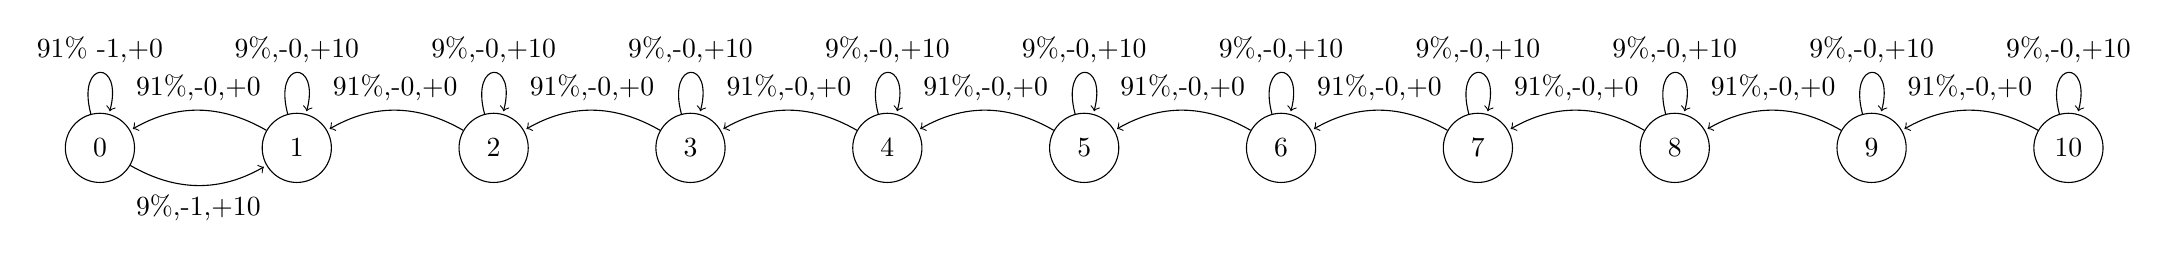
\begin{tikzpicture}

\createNode{0}{0}{0.0}{0.0}{black}{white}
\createNode{1}{1}{2.5}{0.0}{black}{white}
\createNode{2}{2}{5.0}{0.0}{black}{white}
\createNode{3}{3}{7.5}{0.0}{black}{white}
\createNode{4}{4}{10.0}{0.0}{black}{white}
\createNode{5}{5}{12.5}{0.0}{black}{white}
\createNode{6}{6}{15.0}{0.0}{black}{white}
\createNode{7}{7}{17.5}{0.0}{black}{white}
\createNode{8}{8}{20.0}{0.0}{black}{white}
\createNode{9}{9}{22.5}{0.0}{black}{white}
\createNode{10}{10}{25.0}{0.0}{black}{white}
\createLoop{0}{91\% -1,+0}{black}{black}
\createEdge{0}{1}{9\%,-1,+10}{black}{black}
\createEdge{1}{0}{91\%,-0,+0}{black}{black}
\createLoop{1}{9\%,-0,+10}{black}{black}
\createEdge{2}{1}{91\%,-0,+0}{black}{black}
\createLoop{2}{9\%,-0,+10}{black}{black}
\createEdge{3}{2}{91\%,-0,+0}{black}{black}
\createLoop{3}{9\%,-0,+10}{black}{black}
\createEdge{4}{3}{91\%,-0,+0}{black}{black}
\createLoop{4}{9\%,-0,+10}{black}{black}
\createEdge{5}{4}{91\%,-0,+0}{black}{black}
\createLoop{5}{9\%,-0,+10}{black}{black}
\createEdge{6}{5}{91\%,-0,+0}{black}{black}
\createLoop{6}{9\%,-0,+10}{black}{black}
\createEdge{7}{6}{91\%,-0,+0}{black}{black}
\createLoop{7}{9\%,-0,+10}{black}{black}
\createEdge{8}{7}{91\%,-0,+0}{black}{black}
\createLoop{8}{9\%,-0,+10}{black}{black}
\createEdge{9}{8}{91\%,-0,+0}{black}{black}
\createLoop{9}{9\%,-0,+10}{black}{black}
\createEdge{10}{9}{91\%,-0,+0}{black}{black}
\createLoop{10}{9\%,-0,+10}{black}{black}
\end{tikzpicture}
\end{document}

